% This file was created with tikzplotlib v0.10.1.
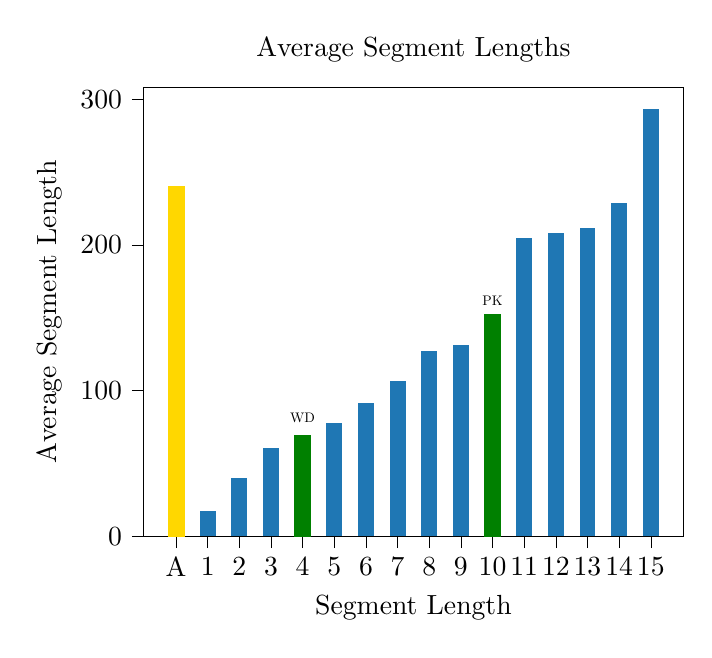
\begin{tikzpicture}

\definecolor{darkgray176}{RGB}{176,176,176}
\definecolor{gold}{RGB}{255,215,0}
\definecolor{green}{RGB}{0,128,0}
\definecolor{steelblue31119180}{RGB}{31,119,180}

\begin{axis}[
tick align=outside,
tick pos=left,
title={Average Segment Lengths},
x grid style={darkgray176},
xlabel={Segment Length},
xmin=-1.025, xmax=16.025,
xtick style={color=black},
xtick={0,1,2,3,4,5,6,7,8,9,10,11,12,13,14,15},
xticklabels={A,1,2,3,4,5,6,7,8,9,10,11,12,13,14,15},
y grid style={darkgray176},
ylabel={Average Segment Length},
ymin=0, ymax=307.940922620857,
ytick style={color=black}
]
\draw[draw=gold,fill=gold] (axis cs:-0.25,0) rectangle (axis cs:0.25,240.25321888412);
\draw[draw=none,fill=steelblue31119180] (axis cs:0.75,0) rectangle (axis cs:1.25,17.0158770288258);
\draw[draw=none,fill=steelblue31119180] (axis cs:1.75,0) rectangle (axis cs:2.25,39.7884628563389);
\draw[draw=none,fill=steelblue31119180] (axis cs:2.75,0) rectangle (axis cs:3.25,60.3045271684641);
\draw[draw=green,fill=green] (axis cs:3.75,0) rectangle (axis cs:4.25,68.8175305659156);
\draw[draw=none,fill=steelblue31119180] (axis cs:4.75,0) rectangle (axis cs:5.25,77.8579323970508);
\draw[draw=none,fill=steelblue31119180] (axis cs:5.75,0) rectangle (axis cs:6.25,91.7970735831732);
\draw[draw=none,fill=steelblue31119180] (axis cs:6.75,0) rectangle (axis cs:7.25,106.903518428513);
\draw[draw=none,fill=steelblue31119180] (axis cs:7.75,0) rectangle (axis cs:8.25,127.009069045054);
\draw[draw=none,fill=steelblue31119180] (axis cs:8.75,0) rectangle (axis cs:9.25,131.601967050093);
\draw[draw=green,fill=green] (axis cs:9.75,0) rectangle (axis cs:10.25,151.904432162218);
\draw[draw=none,fill=steelblue31119180] (axis cs:10.75,0) rectangle (axis cs:11.25,204.553440485213);
\draw[draw=none,fill=steelblue31119180] (axis cs:11.75,0) rectangle (axis cs:12.25,208.062876575439);
\draw[draw=none,fill=steelblue31119180] (axis cs:12.75,0) rectangle (axis cs:13.25,211.490645359217);
\draw[draw=none,fill=steelblue31119180] (axis cs:13.75,0) rectangle (axis cs:14.25,228.909763395417);
\draw[draw=none,fill=steelblue31119180] (axis cs:14.75,0) rectangle (axis cs:15.25,293.277069162721);
\draw (axis cs:4,75) node[
  scale=0.5,
  anchor=south,
  text=black,
  rotate=0.0
]{WD};
\draw (axis cs:10,155) node[
  scale=0.5,
  anchor=south,
  text=black,
  rotate=0.0
]{PK};
\end{axis}

\end{tikzpicture}
